\chapter{Simulation}
Output measurement with harmonic balance simulator in agilent design system in time domain for different signal bandwidths (e.g. \SI{125}{\MHz}, \num{500e6} Hz, 1GHz). The transistor models used in agilents design system was generated at IAF. Which exact model?\\
Three different signals are simulated using this digital-to-analog converter. These signals were generated with a resolution of 3-bit a oversampling ratio of four and the generated signal bandwidth is depending on the control frequency.
All signals are generated using a oversampling ratio of four, $OSR = 2^{r} = 4$. Hence the factor $r = 2$ which is used in the diagrams provided by the french mathematics. The digital control sequence is based on the weights of the slopes and the riemann code is generated by hand. Therefore no MATLAB script exists which calculates the optimal code, minimizing the error, for controlling the digital to analog converter. 
\begin{enumerate}
	\item Vout simulation: three-bit resolution, osr = 4, BW limits: DC to 6GHz$\rightarrow$ could not be processed, manufactured while the period of the thesis. 
	\begin{itemize}
		\item sine ;produce every signal out of sine wave (fourier transformation)
		\item half sine ;only as an example
		\item triangular ;only as an example
	\end{itemize}
	\item Vout simulation: two-bit resolution, osr = 4, keep it small and simple, frequency higher, demonstrator, assembly, less complex
	\begin{itemize}
		\item sine
		\item half sine ;only as an example
		\item triangular ;only as an example
	\end{itemize}
	\item S-parameter		
	\item Switch voltage
	\item Max Gain with output amp
	\item stability
	\item energy consumption
\end{enumerate}
Explain Bandwidth limitations. The lower bound is determined by the sampling time (inverse of the sampling frequency;) and the smallest current achieved with the dimensioned transistors. The smallest achievable current times the smallest sampling time (highest sampling frequency) determine the smallest absolute slope achievable. \\ \textbf{Is every signal possible to create? The signal bandwidth ranges from DC to 6 GHz but what is the amplitude range? Is there a limitation regarding the amplitude?}
\\
The smallest current is determined by the dimension of the transistor, which drives into saturation. The smallest saturated current is determined by the push-pull transistor geometry, here: 532 mA.\\Voltage across capacitor is determined by:
\begin{equation}
U = \frac{1}{C} \int I  dt 
\end{equation}

\begin{itemize}
	\item Harmonic Balance simulation is used to neglect the transient time (steady-state)
	\item S-parameter simulation is done for the matching, determining impedance
	\item Stability simulation is done to check whether or not oscillation occurs
	\item energy consumption is determined by the HB simulation; more or less
\end{itemize}

%% Important: appearance(format) all the same, same frequency, sam oversamplingratio, same resolution, et cetera
% create this figure/picture
%\begin{figure}[ht]
%	\centering
%  \includegraphics[width=1\textwidth, draft]{DAC_generated_sine_wave.png}
%	\caption{Digital to analog converted signal representing a sine wave using ads simulation}
%	\label{DAC_generated_sine_wave}
%\end{figure}

\section{time signal simulation with three bit resolution dac}
A theoretical created sine wave is compared to the synthesized sine wave with the riemann pump simulation. As seen in Figure \ref{fig:SineCompare} the synthesized signal is very close to the theoretical optimal. The deviation is very small hence the signal to noise ratio is very low. As in equation \ref{eq:SNR_RiemannPumpConversion} stated the snr is calculated.
\begin{figure}[ht]
	\centering
  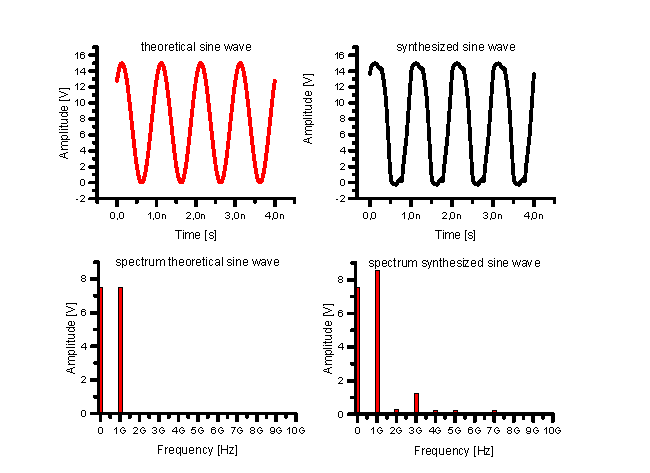
\includegraphics[width=1\textwidth]{SineCompare.pdf}
	\caption{Comparison between a theoretical and a synthesized sine wave with their spectrum}
	\label{fig:SineCompare}
\end{figure}

Figure \ref{fig:1GHz sine} shows a sine wave with a frequency of 1 GHz synthesized with the DAC. The control frequency is eight times the signal bandwidth.
\begin{figure}[htb]
   \centering
   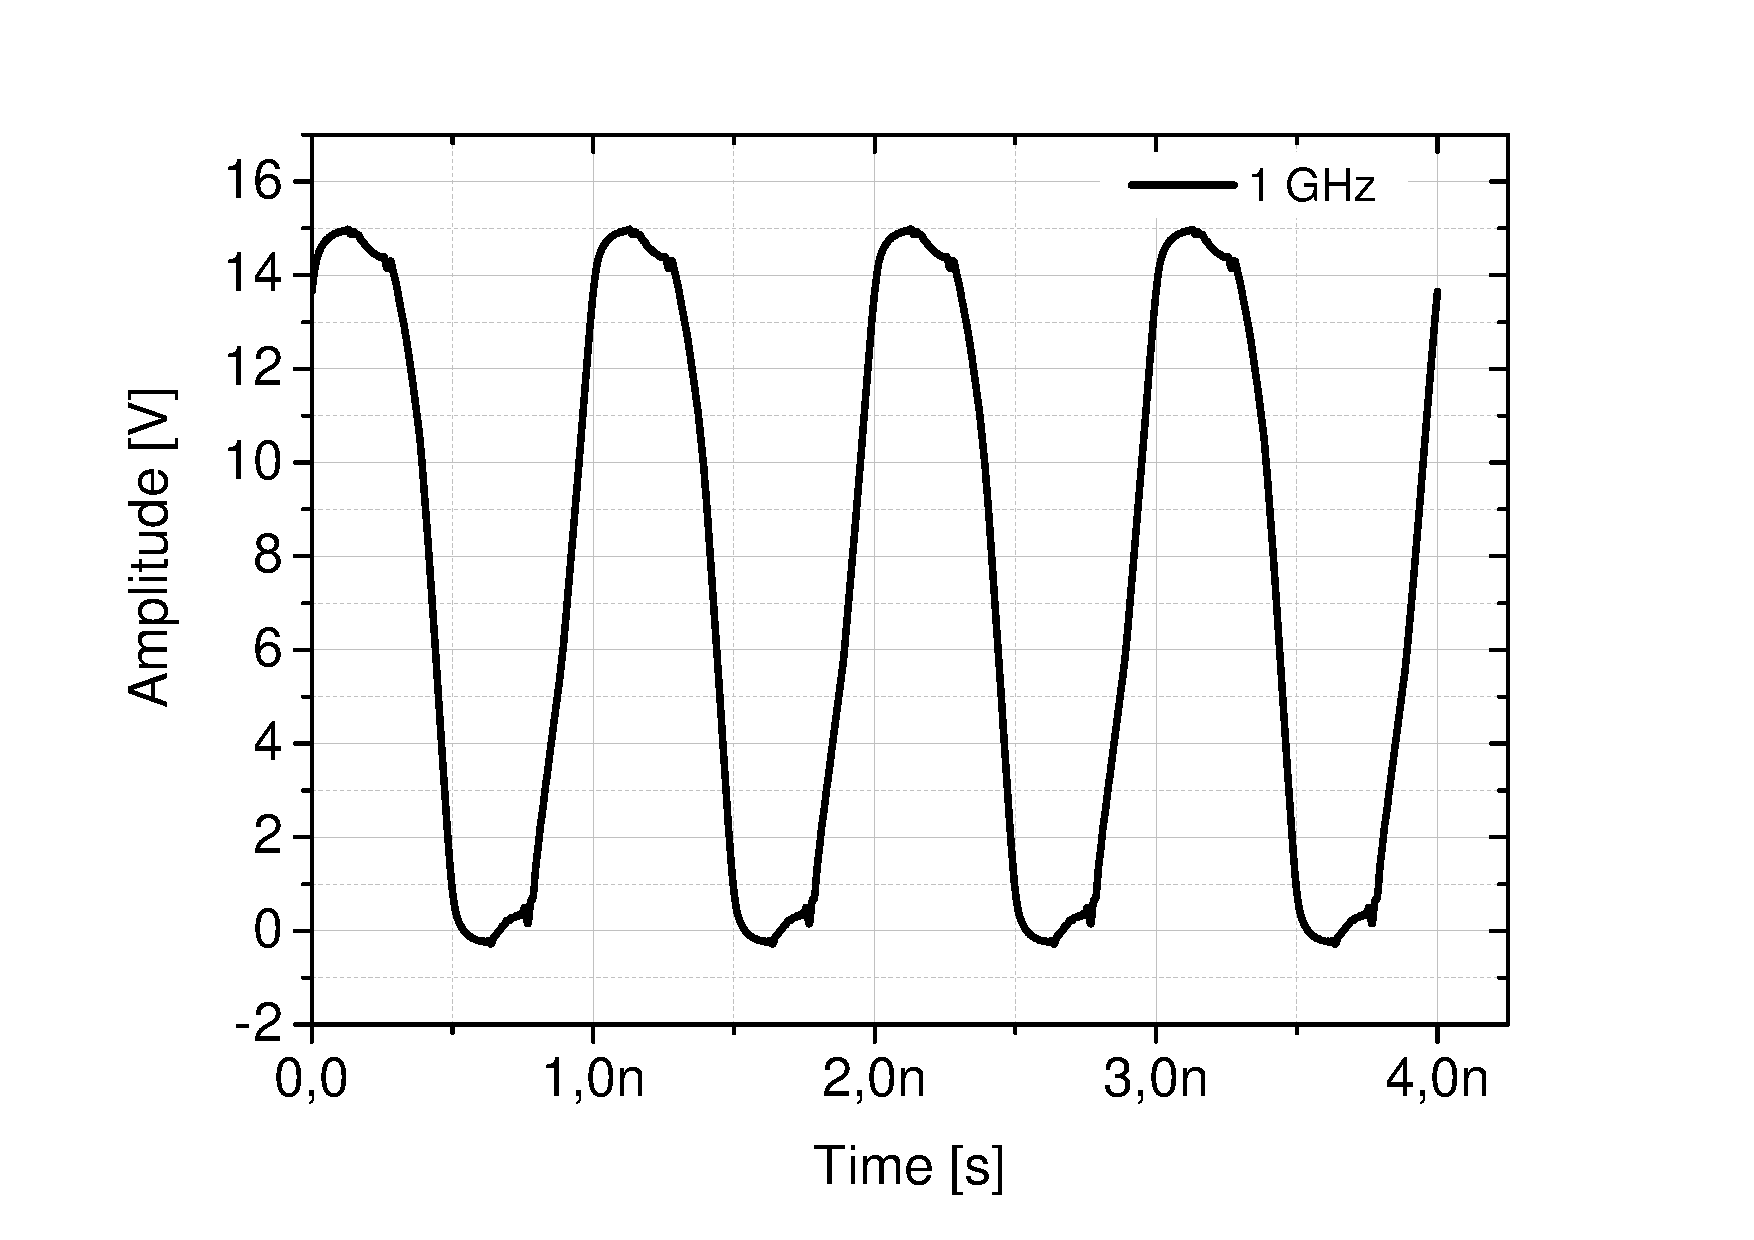
\includegraphics[width=0.75\textwidth]{Vout_sine_SigBW_1GHz_3bit_long.pdf}
   \caption{amplitude of a synthesized sine wave with signal frequency of 1 GHz, $f_{sampling} =$ \SI{8}{\GHz} in the time domain}
   \label{fig:1GHz sine}
\end{figure}
This signal is generated with the riemann code. This riemann code was obtained by hand with optical estimation with the slopes obtained from the table.

\begin{figure}
\centering
\begin{minipage}{.5\linewidth}
  \centering
  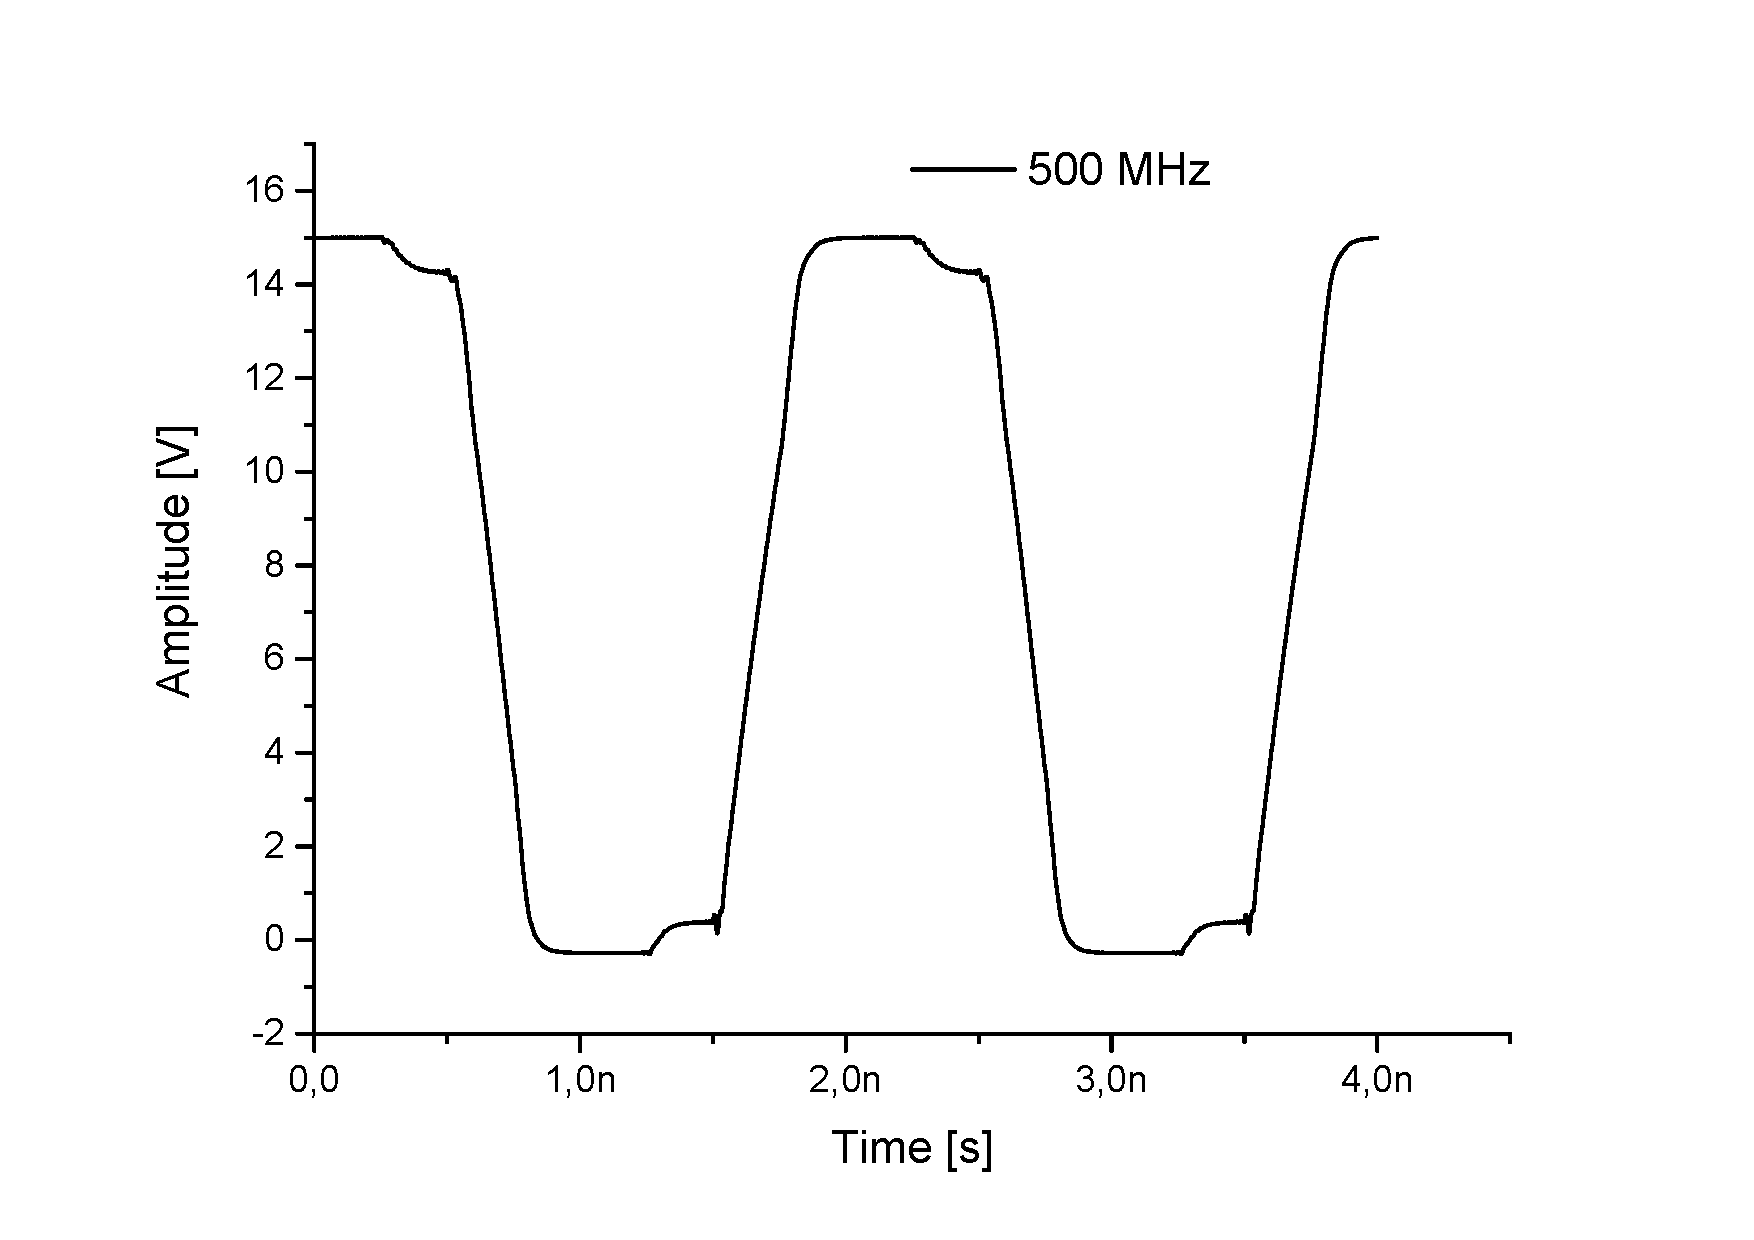
\includegraphics[width=1\linewidth]{Vout_sine_SigBW_05GHz_3bit.pdf}
  %\caption{500 MHZ signal}
  \label{fig:test1}
\end{minipage}%
\begin{minipage}{.5\linewidth}
  \centering
  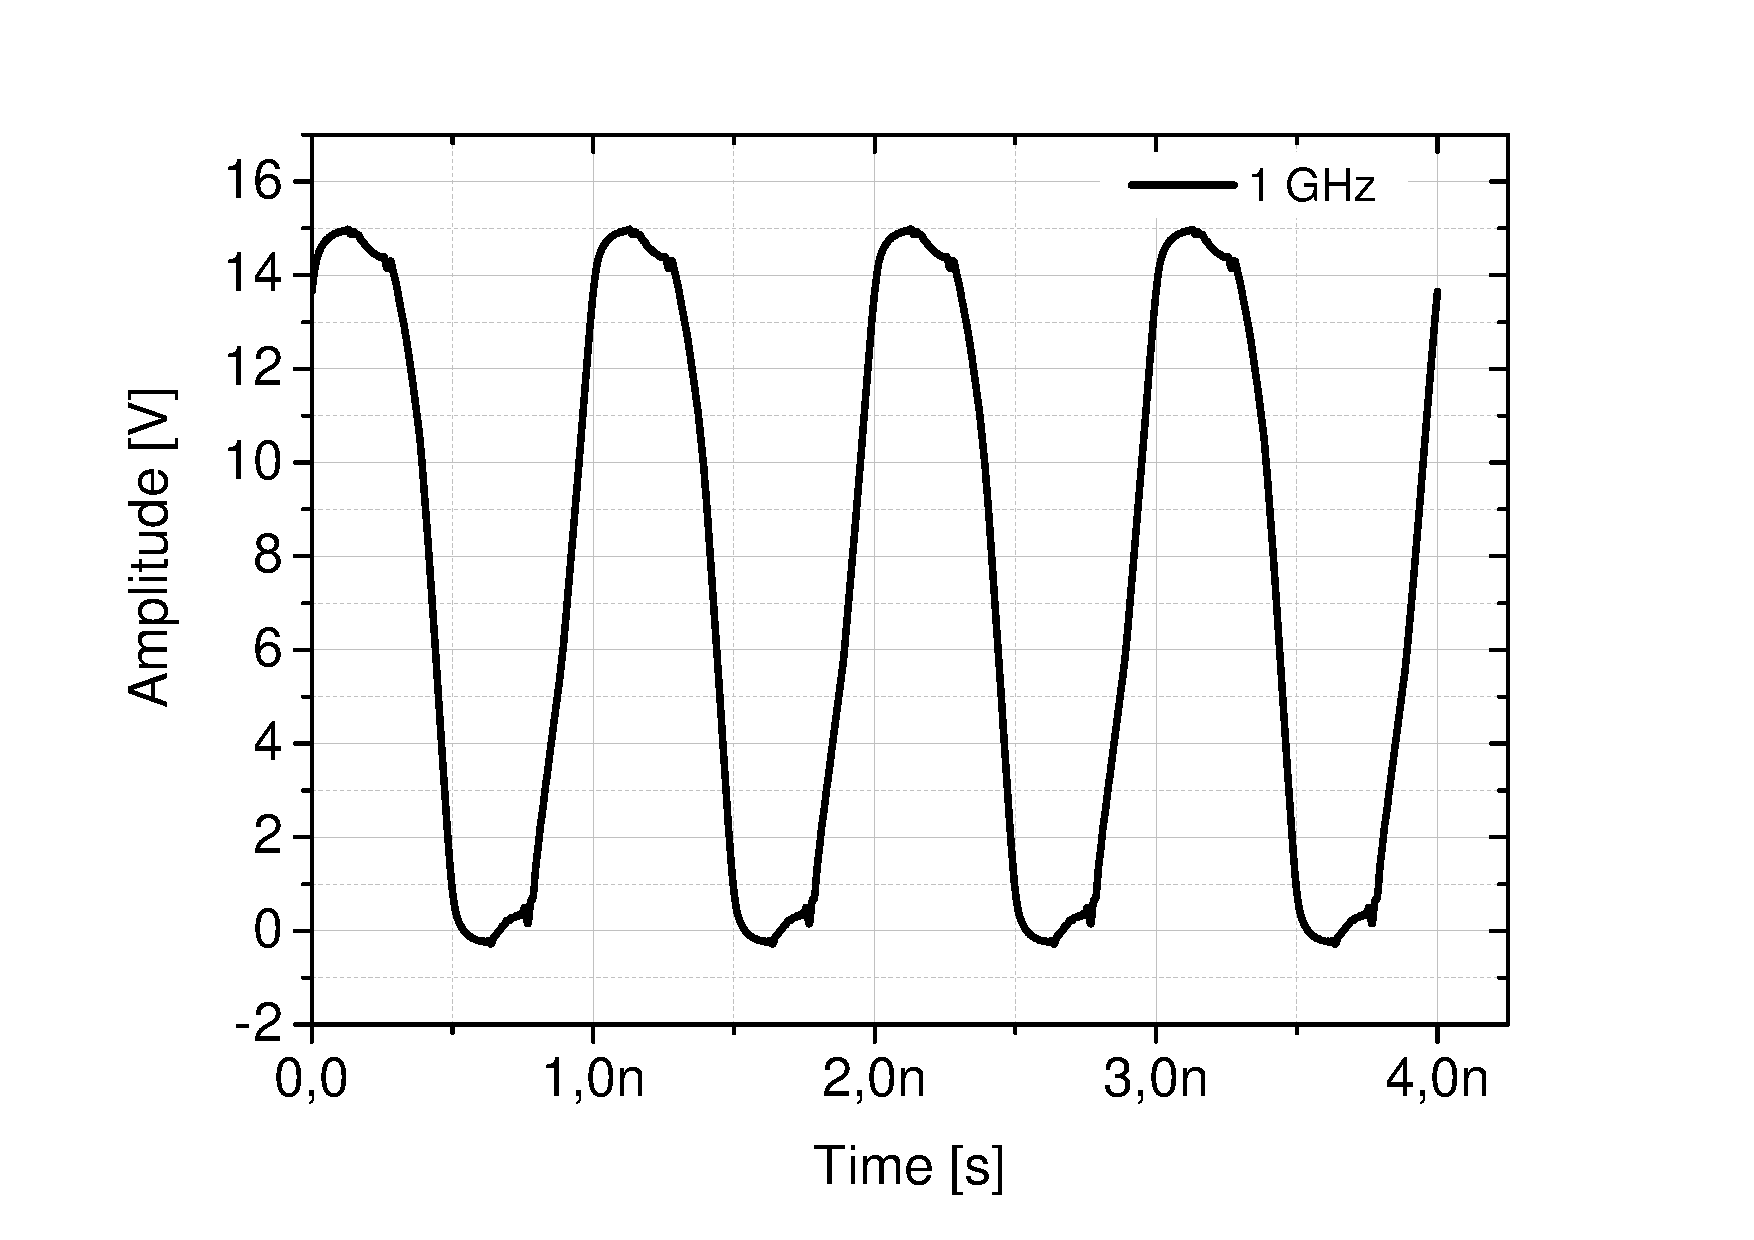
\includegraphics[width=1\linewidth]{Vout_sine_SigBW_1GHz_3bit_long.pdf}
  %\caption{2 GHz}
  \label{fig:test2}
\end{minipage}
%\end{figure}
%
%
%\begin{figure}
\centering
\begin{minipage}{.5\linewidth}
  \centering
  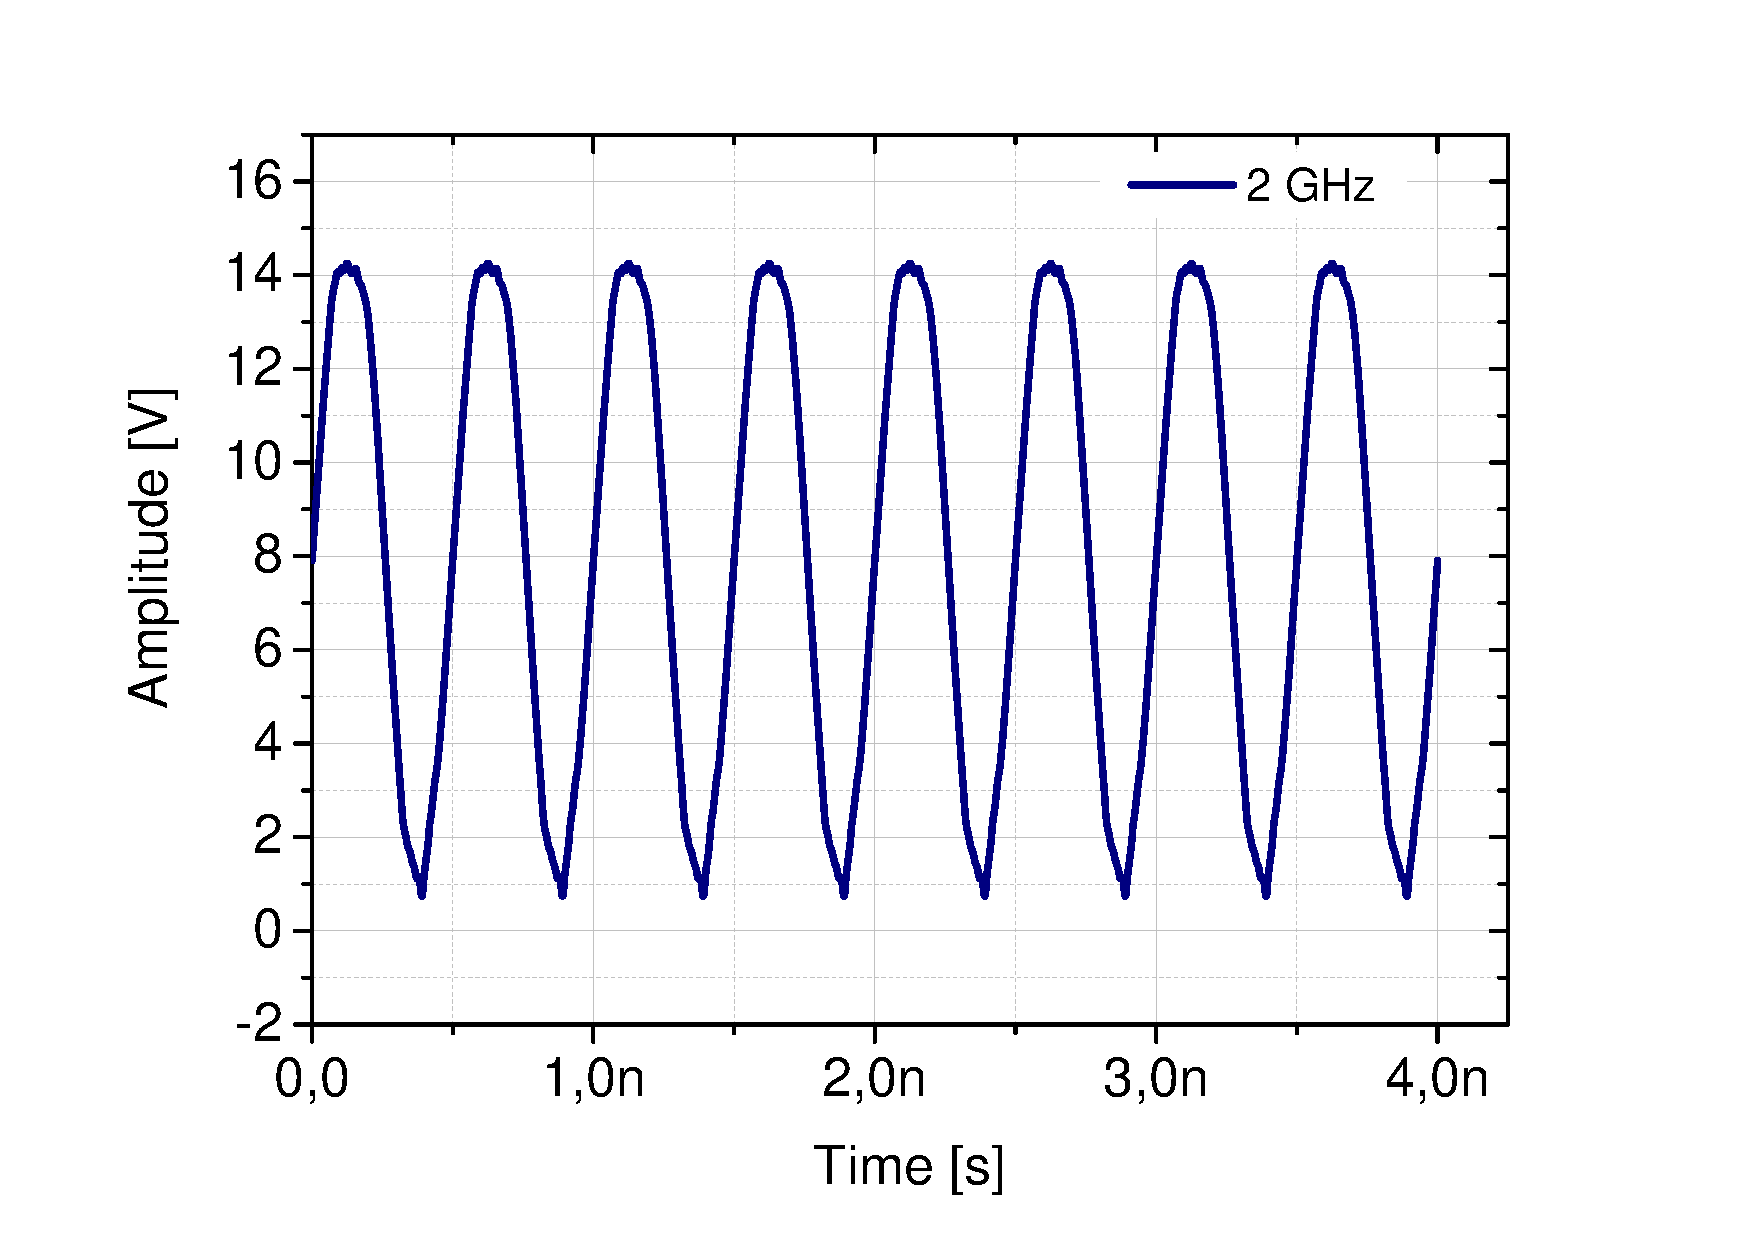
\includegraphics[width=1\linewidth]{Vout_sine_SigBW_2GHz_3bit_long.pdf}
 % \caption{1GHZ signal}
  \label{fig:test3}
\end{minipage}%
\begin{minipage}{.5\linewidth}
  \centering
  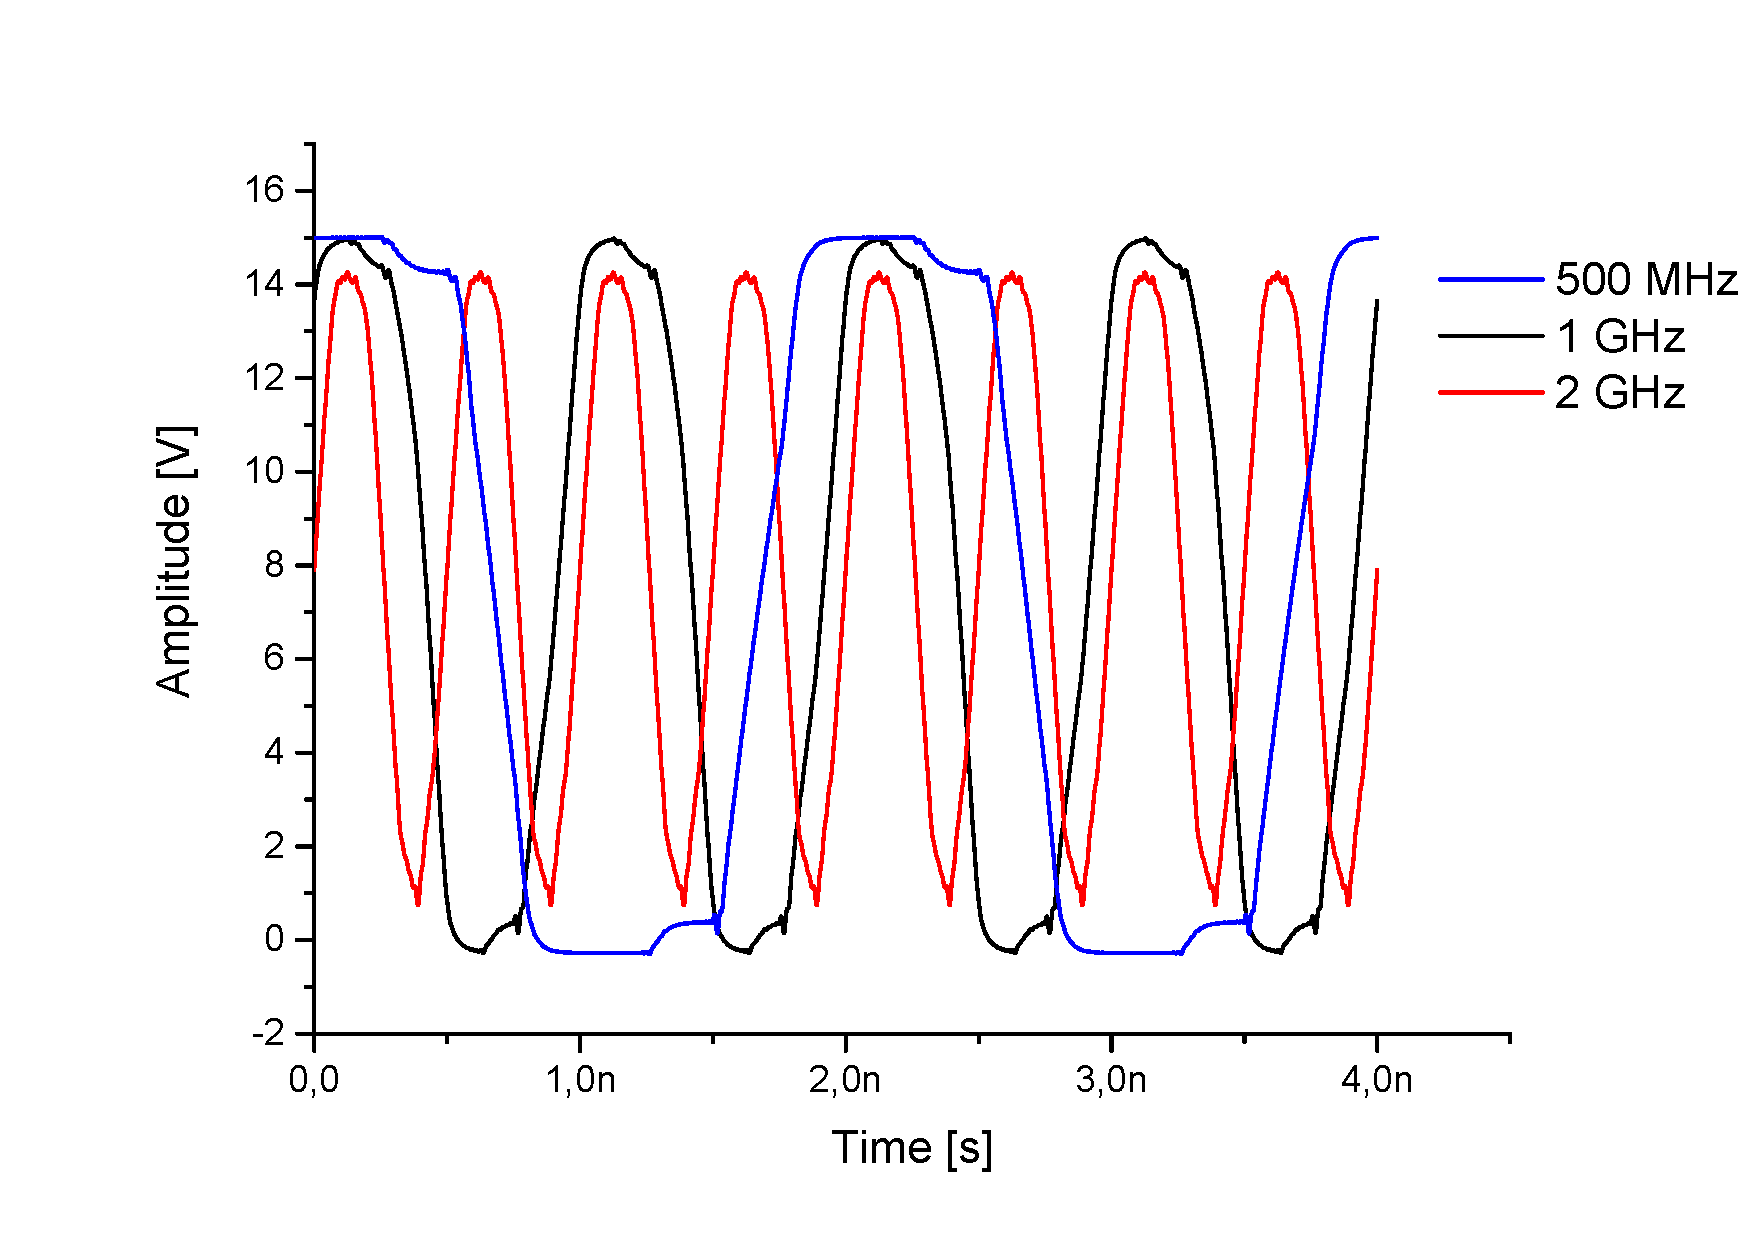
\includegraphics[width=1\linewidth]{Vout_sine_SigBW_ALL_3bit.pdf}
%  \caption{2 GHz}
  \label{fig:test4}
\end{minipage}
\end{figure}


\section{time signal simulation with two bit resolution dac}
\subsection{time signal simulation with optimized geometry for transistor}
\subsection{demonstrator based simulation}
